% !TeX root = ../main.tex

\chapter{Motivation}\label{chapter:Motivation}

In todays world, all software that has been developed by a team of programmers is bound to have errors, and the amount of them you might have in a project will only keep incrementing if they are not dealt with in a timely manner. Of all these errors that are found, they usually lead to vulnerabilities in our system, which can be exploted in several ways -- ways which will be discussed at a later point in this thesis -- and sometimes the time to fix one vulnerability completely outweights the benefit provided. That is why knowing the severity of a given vulnerability is usualy crucial to assess correctly the amount of resources we need to assign for its correction.

\section{Vulnerabilities}
Since the inception of informatics, errors in code, be it semmantic or synactic, have existed. These errors, as mentioned previously, usually lead to security issues in our application, called software vulnerabilities.

Most errors arise from simple programming mistakes, and vary from one programing language to another, as well as the field where these programms are being put to use. Regardless of how a vulnerability comes to be, a solution needs to be found for it, which usually includes its development, testing, and a deployment.

But in projects where there are more vulnerabilities than resources to assign to them, or when fixing one vulnerability would yield a benefit that is simply not worth the investment? What if there was a way to include a numerical approximation that assesses its severity? We go into detail throughout this chapter, covering all of the reasons that lead us to undertake this project.

\subsection{How are vulnerabilities found}

A vulnerability can be found in a pleathora of ways: it can be a simple semicolon missing from the code, it could be a typo in one variable, these are now-a-days easy to find since there are IDEs (Integrated Development Environment); or it could be that someone overlooked sanitizing an input, that could lead to buffer-overflow errors during runtime. Whichever the source of a given vulnerability, the approach to find a it is always the same: reproduce this error by supplying the inputs that got the software to an unstable state, or in most cases, crashed it.

There are tools and methodologies to automize the process of discovering vulnerabilities, by testing the program's correctness, optimization, verification, performance, profiling, etc. In our thesis we have decided to opt for symbolic execution as a means of finding vulnerabilities in an automatic manner. The difference of symbolic execution against other types of analysis such as static, or dynamic is that, for instance in a function that would normally receive two integers as its parameters, now receives two symbols, that can take any value possible from the range of integers, thus testing all possible combinations, and testing all possible scenarios, in contrast to static or dynamic were specific values are passed and compared to an expected final state set by us. What symbolic execution provides is a thorough analysis of programs, such that will try to discover vulnerabilities in all possible branches of a given program, whenever a program can be analysed with the proper tools.

\subsubsection{Buffer-overflow vulnerabilities}

\todo{HERE}

\subsection{The severity of a vulnerability}

A vulnerability has the power to bring a whole system down. They can be a force to be reckoned with, when it has spawned inside a codebase that has built up to millions of lines of code. After a vulnerability has been found, we must know how severe its impact on the system will be, and act accordingly. If a severity has the power of bringing the system down, we know it is quite severe. 

But what happens in the normal occation when a vulnerability is found and there is no way to know how severe it is at first glance? when there are several vulnerabilities that subjectively speeking, all seem to affect the system equally? When resources are scarse and we need to prioritize which vulnerability to focus on next so that our system may continue working as inteded?
When there are extremely huge time constraints and we can only budget to fix one at a time, because our workforce is limited?

\subsection{Common Vulnerability Scoring System}

The Research by the National Infrastructure Advisory Council (NIAC) in 2003/2004 led to the launch of CVSS version 1 in February 2005, with the goal of being "designed to provide open and universally standard severity ratings of software vulnerabilities". This initial draft had not been subject to peer review or review by other organizations. In April 2005, NIAC selected the Forum of Incident Response and Security Teams (FIRST) to become the custodian of CVSS for future development. 

FIRST.Org, Inc. (FIRST), a US-based non-profit organization, whose mission is to help computer security incident response teams across the world\parencite{cvss3} asked themselves these same questions back in 2005, when they decided to introduce CVSS, or Common Vulnerability Scoring System\parencite{cvss3}.

Throughout this thesis we introduce ways to find the severity of a specific vulnerability. Depending on several values, and using the aforementioned metric CVSS3 as our basis to rate them, we will give a vulnerability a numeric score, which could allow us to know what vulnerability should be given priority, and which one might be harmless.

\section{Symbolic execution}

Symbolic execution is a way of testing a program to determine what inputs allow the software to execute. Instead of using normal variables for testing, an interpreter follows the execution assuming symbolic values as the inputs instead of using concrete values -- as per in normal execution -- which can take any value for the given type of the input, thus covering the complete range of possible branches the program could take, therefore discovering vulnerabilities along its way.


\subsection{Modular and Compositional Analysis with KLEE Engine}

Throughout this thesis MACKE (Modular and Compositional Analysis with KLEE Engine)\parencite{ognawala} will be used to find vulnerabilities, and callgraphs of programs to fully analize the source of the vulnerability, and the possible severity of it.

This tool makes use of symbolic execution techniques at the level of C functions, and then combines the results using static code information and inter-procedural path feasibility\parencite{ognawala}.

The use of this tool allows us to find an extensive amount of undocumented and documented bugs. The documented bugs found will be analyzed in the initial phases, since they have already been assessed manually with the CVSS3 framework.

\section{Callgraphs}

A callgraph\parencite{dataFlow} is the relationship between functions in a computer program, where several functions are present. It is, for the most part, user readable, and allows for an overall view of a program. It helps to pinpoint functions that might be unused, and if there are a few functions that are too intertwined. In general, a callgraph allows users to find if the intended purpose of the program has been met, and if the means to achieve the result was correct.

\begin{figure}[!htb]
	\caption{Program callgraph}
	\centering
	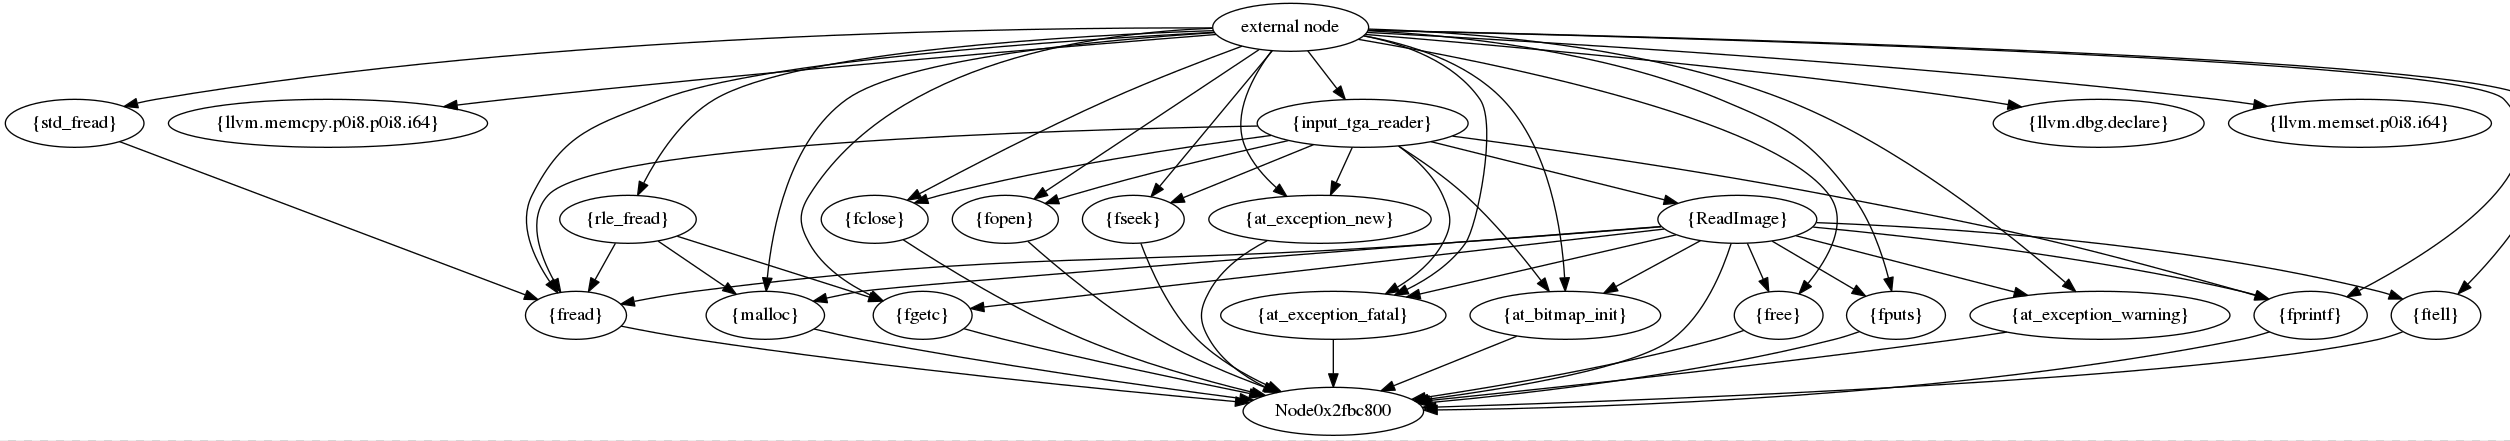
\includegraphics[width=1.0\textwidth]{callgraph1}
\end{figure}

\subsection{Callgraph types}

Call graphs can be dynamic or static. A dynamic call graph is a record of an execution of the program, for example as output by a profiler. Thus, a dynamic call graph can be exact, but only describes one run of the program. A static call graph is a call graph intended to represent every possible run of the program. The exact static call graph is an undecidable problem, so static call graph algorithms are generally overapproximations. That is, every call relationship that occurs is represented in the graph, and possibly also some call relationships that would never occur in actual runs of the program.

Call graphs can be defined to represent varying degrees of precision. A more precise call graph more precisely approximates the behavior of the real program, at the cost of taking longer to compute and more memory to store. The most precise call graph is fully context-sensitive, which means that for each procedure, the graph contains a separate node for each call stack that procedure can be activated with. A fully context-sensitive call graph is called a calling context tree. This can be computed dynamically easily, although it may take up a large amount of memory. Calling context trees are usually not computed statically, because it would take too long for a large program. The least precise call graph is context-insensitive, which means that there is only one node for each procedure.


\section{Putting it all together}

By using compositional symbolic execution we would be able to find some vulnerabilities -- as many as MACKE can find in its scope of testing -- and also generate the programs callgraph. By having these two components, and by measuring its vulnerability -- by following the CVSS3 guidelines -- we could correlate the graph attributes to each and every one of the base scores, to see if there is a pattern, which could later then be used to generate a supervised learning algorithm that could automatically give us the CVSS3 scores of bugs found by MACKE. 

The main drive behind doing this is the belief that the relations among functions, and their location in the graph is deeply intertwined with the severity of a vulnerability. A callgraph can tell us if the program is accessible directly, or not, for instance. It can also tell us if a vulnerability will prograpate or not, allowing us to pinpoint the starting and end points of a potential chain of errors.



